\chapter{Felhasználói dokumentáció}
\label{ch:user}


\section{A szoftver célja}

Az alkalmazásnak három fő célja van:
\begin{enumerate}
    \item Biztosítani egy szerkesztőt, amivel bármilyen 2D-s sokszög elkészíthető.
    \item Lehetőséget adni arra, hogy az elkészített poligonon lefuttassuk az algoritmust.
    \item Személyreszabható és látványos módon vizualizáni a kiértékelt távolságfüggvényt
\end{enumerate}


\section{Hardveres és szoftveres követelmények}

\textbf{Hardver}
\begin{itemize}
    \item x86-64 architektúrájú CPU (Modern Intel vagy AMD processzorok többsége)
    \item DirectX 12 API kompatibilis GPU
    \item 8GB RAM
    \item billentyűzet, egér, monitor
\end{itemize}

\textbf{Szoftver}
\begin{itemize}
    \item Operációs rendszer: Windows 11
    \item DirectX 12 API kompatibilis GPU driver
\end{itemize}


\section{Telepítés és futtatás}

A program nem rendelkezik telepítővel, a mellékelt állomány kicsomagolása után a \textit{"PolygonSDF.exe"} futtatásával azonnal használható. A mellékelt fájlok és mappák (pl. \textit{Falcor.dll}, \textit{Shaders/}, \textit{Data/}, ...) szükségesek az alkalmazás megfelelő működéséhez.


\section{Szerkesztői nézet}

Az alkalmazás indítása után a felhasználót a szerkesztői nézet fogadja, amelyben egy előre meghatározott poligon jelenik meg. Egy poligon több "alpoligonból" áll, minden alpoligont annak csúcspontjaival adjuk meg, ahol a megadási sorrend határozza meg azt, hogy hogy kötjük őket össze. A távolság előjelét az határozza meg, hogy az adott pont páros vagy páratlan számú sokszögön belül van-e, ami páros esetén pozitív és páratlan esetén negatív távolságot eredményez.

A szerkesztőben lehetőségünk van alpoligonok felvételére, mozgatására és törlésére, valamint csúcspontjaik módosítására. Ezen műveleteket kétféle módon is elvégezhetjük, a vizuális szerkesztővel, a billentyűzet és egérmozdulatok segítségével, vagy a GUI-n elhelyezett beviteli mezőkkel és gombokkal. Amikor elkészültünk a szerkesztéssel, az algoritmust is ezen felületen keresztül futtathatjuk le.

\begin{figure}[H]
    \centering
    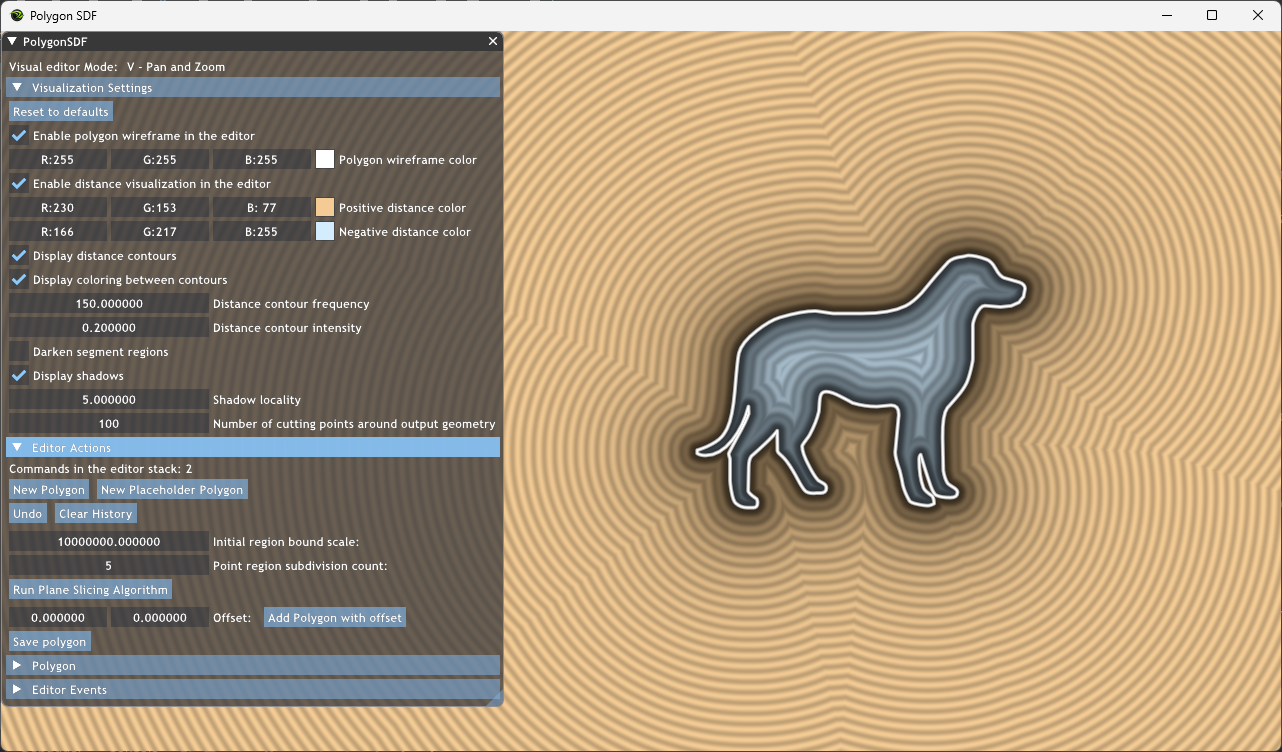
\includegraphics[width=1\linewidth]{images/editor.png}
    \caption{Szerkesztői nézet}
    \label{fig:editor-1}
\end{figure}

\section{GUI szerkesztő}

Lehetővé teszi, hogy pontos értékekkel dolgozzunk a szerkesztés közben, mivel beviteli mezőkkel és gombokkal adunk ki parancsokat kattintások helyett a vásznon.
Ezért GUI szerkesztő központi szerepet tölt be az alkalmazás használatában, bizonyos műveleteket csak itt lehet végrehajtani, mint például a vizualizációs beállítások módosítása, algoritmus lefuttatása, mentés és betöltés. Itt kerül megjelenítésre az is, hogy a vizuális szerkesztő milyen módban van.

A GUI szerkesztő csoportokra van felosztva, az elvégzett feladatkör szerint.


\subsection{Vizualizációs beállítások}

Ebben a szekcióban állíthatjuk be az objektumunk megjelenítését. Bizonyos tulajdonságok, mint például a színezés, árnyékolás, vagy kontúrozás, mindkét nézetben érvényesülnek.

\begin{figure}[H]
    \centering
    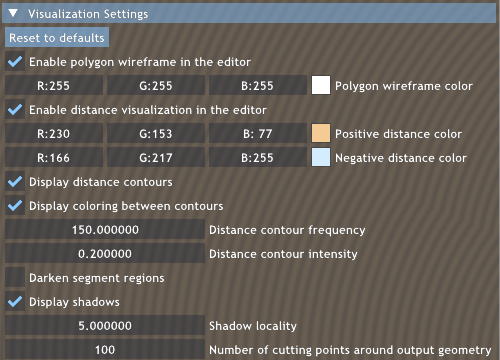
\includegraphics[width=0.8\linewidth]{images/visualization_settings.png}
    \caption{Vizualizációs beállítások GUI}
    \label{fig:visualization_settings-1}
\end{figure}

\textbf{Elérhető beállítások}

\begin{description}
    \item[Körvonal engedélyezése] Ki- és bekapcsolhatjuk a poligon körvonalának megjelenítését.
    \item[Körvonal szín] Kiválaszthatjuk, hogy milyen RGB értékkel kerüljön kirajzolásra a körvonal.
    \item[Távolság megjelenítésének engedélyezése] Szabályozhatjuk, hogy az alkalmazás rajzolja-e a távolságot. Ez egy viszonylag drága beaállítás, mert a minden kiszínezett pixelre a képernyőn ki kell értékelni a távolságot.
    \item[Távolság pozitív tartományának színe] Megadhatjuk, hogy a pozitív tartomány színezésekor milyen alapszínt használjon a program
    \item[Távolság negatív tartományának színe] Megadhatjuk, hogy a negatív tartomány színezésekor milyen alapszínt használjon a program
    \item[Távolsági kontúrok megjelenítése] Kontúrok megjelenítésének szabályozása.
    \item[Kontúrok közötti tartomány kitöltése] Beállítás a kontúrok közötti tartomány színezésére. Amennyiben le van tiltva a kontúrok közötti terület nem kerül színezésre.
    \item[Távolsági kontúrvonalak frekvenciája] A távolság megjelenítéséhez használt kontúrvonalak gyakorisága. A magasabb megadott érték sűrűbben elhelyezkedő kontúrvonalakat eredményez.
    \item[Távolsági kontúrvonalak intenzitása] Megadja, hogy színezéskor mennyivel súlyozzuk a kontúr színét a háttérhez képest. Nulla értékű intenzitással nincsenek kontúrvonalak, egy értéknél pedig nincs színezés közöttük.
    \item[Árnyék megjelenítése] Ki- és bekapcsolhatjuk az árnyékok rajzolását a poligon körvonala mentén. A háromdimenziós nézetben fontos szerepe van az árnyéknak, mert információt ad a geometria mélységéről.
    \item[Árnyék lokalitása] A beállított értékkel megszabhatjuk, hogy mekkora területre terjedjen ki az árnyék. Nagyobb érték esetén az árnyékolt rész kisebb, gyorsabban veszít az intenzitásából, ahogy a távolság növekedik.
    \item[Szakaszokhoz tartozó régiók elsötétítése] Ezzel a beállítással látványosabbá tehetjük azt, hogy egy adott pontban a poligon egy szakaszához, vagy egy csúcsához van-e közelebb. A szakaszokhoz közelebbi pontokhoz tartozó pixelek sötétebb színt kapnak.
    \item[Az algoritmus kimenetének körbevágásához használt pontok száma] Az algoritmus egy \textit{"végtelenül nagy"} síkkal dolgozik. Megjelenítés előtt ezt a síkot az alkalmazás a poligon középpontja körül egy a poligon méretétől függő sugarú körív mentén körbevágja. A beviteli mezővel a vágáshoz használt pontok számát szabályozhatjuk.
\end{description}

\begin{figure}[H]
    \centering
    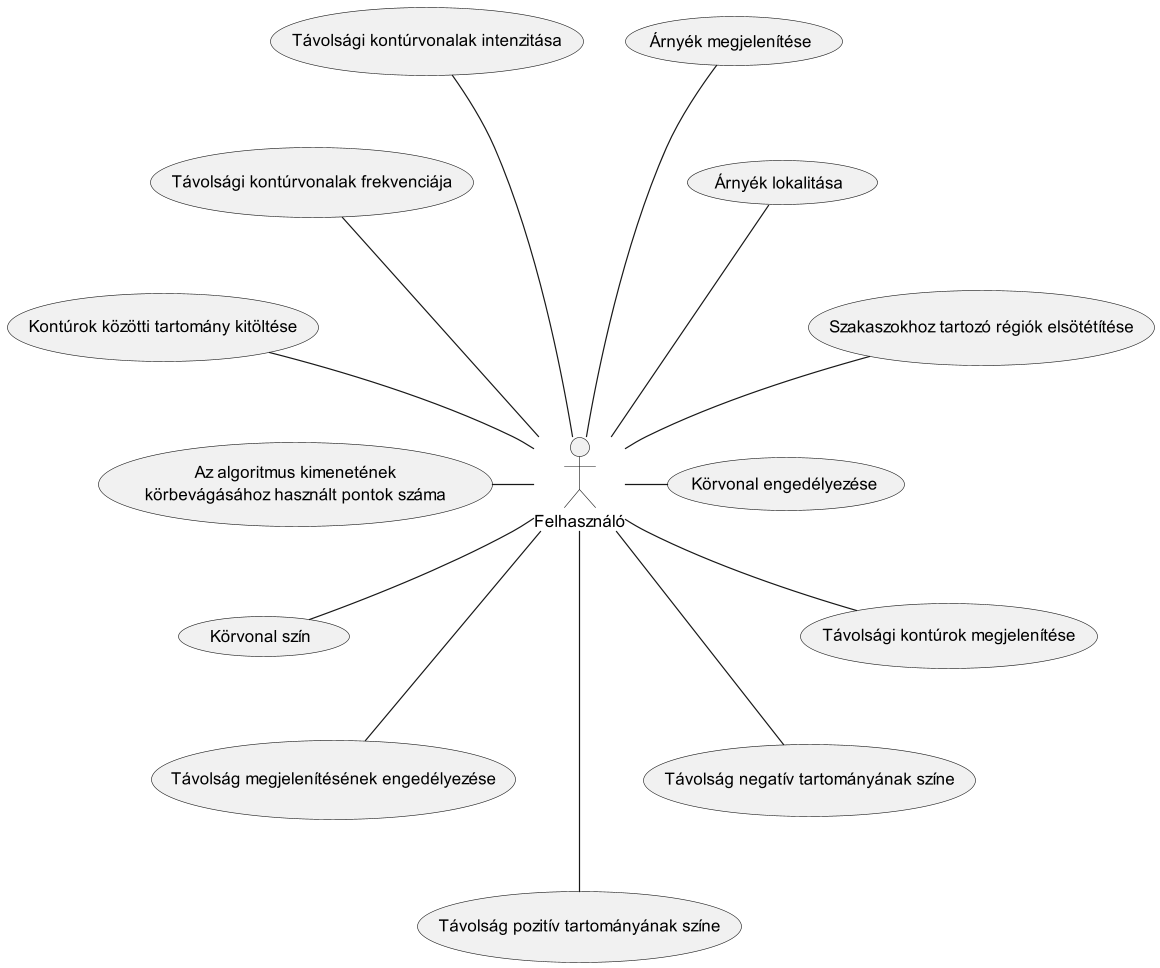
\includegraphics[width=1\linewidth]{images/usecase_visualization_settings.png}
    \caption{Vizualizációs beállítások felhasználói esetek}
    \label{fig:usecase_visualization_settings-1}
\end{figure}

\begin{figure}[H]
    \centering
    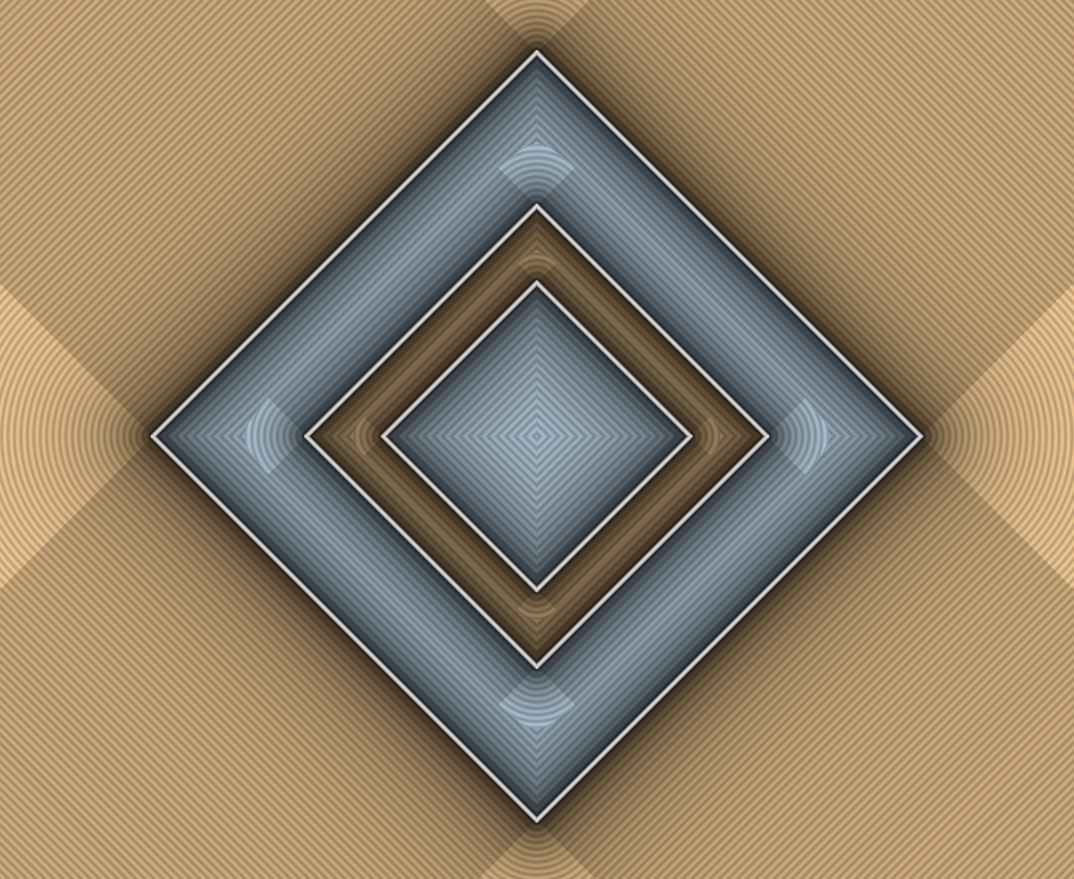
\includegraphics[width=0.85\linewidth]{images/darken_segment_regions.png}
    \caption{Szakaszokhoz tartozó régiók elsötétítése}
    \label{fig:darken_segment_regions-1}
\end{figure}

\begin{figure}[H]
    \centering
    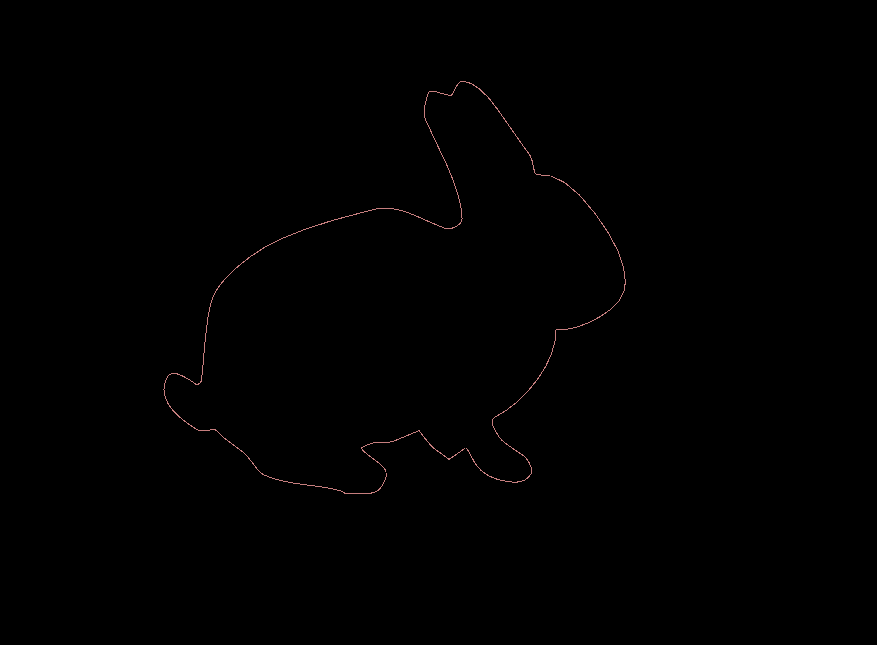
\includegraphics[width=0.85\linewidth]{images/outline_only.png}
    \caption{Poligon "wireframe" nézete}
    \label{fig:outline_only-1}
\end{figure}

\begin{figure}[H]
    \centering
    
\includegraphics[width=0.78\linewidth]{images/hidden_contours.png}
    \caption{Megjelenítés kontúrok nélkül}
    \label{fig:hidden_contours-1}
\end{figure}

\begin{figure}[H]
    \centering
    
\includegraphics[width=0.78\linewidth]{images/low_shadow_locality.png}
    \caption{Megjelenítés alacsony árnyék lokalitással}
    \label{fig:low_shadow_locality-1}
\end{figure}

\begin{figure}[H]
    \centering
    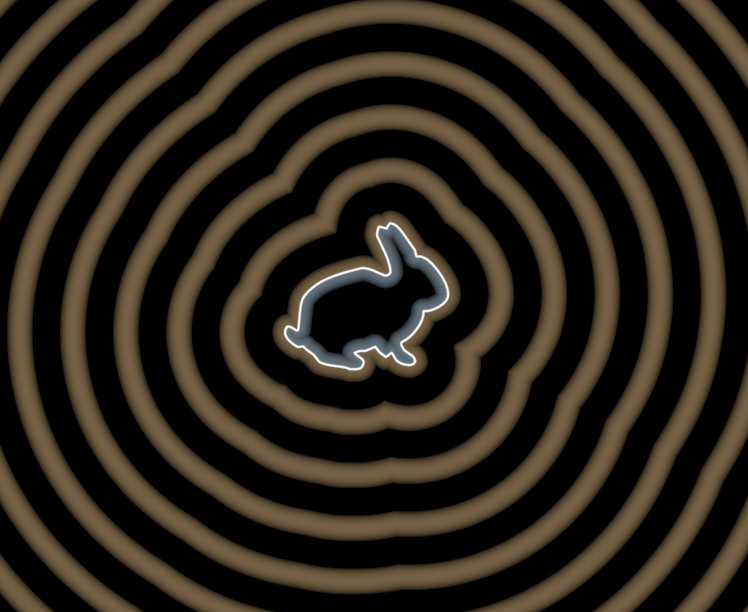
\includegraphics[width=0.85\linewidth]{images/low_contour_frequency.png}
    \caption{Megjelenítés alacsony kontúr frekvenciával}
    \label{fig:low_contour_frequency-1}
\end{figure}

\begin{figure}[H]
    \centering
    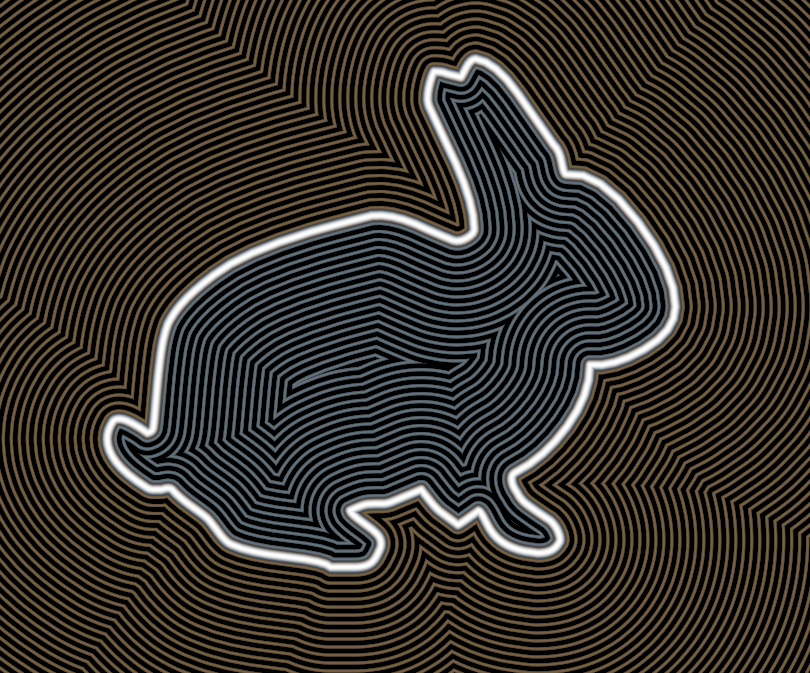
\includegraphics[width=0.85\linewidth]{images/high_contour_frequency.png}
    \caption{Megjelenítés magas kontúr frekvenciával}
    \label{fig:high_contour_frequency-1}
\end{figure}

\subsection{Szerkesztői műveletek}

Ezen szekció alatt általános szerkesztői műveletek találhatóak, mint például adatok betöltése, mentése, algoritmus futtatása. A szerkesztő az állapotokat veremszerűen tárolja, új művelet hozzáadásakor beszúrunk egy új bejegyzést, visszalépéskor pedig kiveszünk egyet. Ez a funkció szabadságot ad a felhasználónak kísérletezésre, mivel bármikor visszaléphet az arra szánt gomb megnyomásával, viszont a műveletek számával növekszik a memóriaigénye is a programnak, ezen a felületen keresztül törölhetjük is a szerkesztői előzményeket.

\begin{figure}[H]
    \centering
    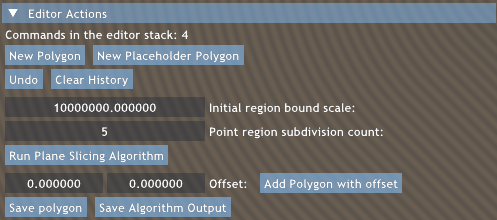
\includegraphics[width=0.85\linewidth]{images/editor_actions.png}
    \caption{Szerkesztői műveletek GUI}
    \label{fig:editor_actions-1}
\end{figure}

\textbf{Elérhető funckionalitás}

\begin{description}
    \item[Új poligon hozzáadása] A fáljrendszerből tölt be egy sokszöget a meglévőt lecserélve, amennyiben a megadott JSON file a megfelelő formátumban van, ellenkező esetben egy felugró ablakkal értesül a felhasználó, hogy a művelet sikertelen.
    \item[Új kezdőpoligon] A jelenlegi poligont lecseréli a kezdőpoligonra.
    \item[Visszalépés] Az utolsó lépés visszavonása, amennyiben lehetséges.
    \item[Előzmények törlése] A szerkesztői előzmények törlése, a köztes állapotokra fenntartott memória felszabadításához.
    \item[A vágásokat végző algoritmus futtatása] Ha a poligon megfelel az algoritmus előfeltételének, tehát nincsenek egymást metsző vagy egymásba eső szakaszok, akkor az alkalmazás végrehajtja. Ellenkező esetben egy felugró ablak jelzi, hogy a művelet sikertelen.
    \item[Poligon hozzáfűzése eltolással] A fáljrendszerből tölt be egy sokszöget a meglévőhöz hozzáfűzve azt, a megadott X és Y koordinátákkal eltolva. Amennyiben a megadott JSON file a megfelelő formátumban van, ellenkező esetben egy felugró ablakkal értesül a felhasználó, hogy a művelet sikertelen.
    \item[Poligon mentése] A szerkesztett poligon jelenlegi állapotát a fáljrendszerbe menti JSON formátumban.
    \item[Algoritmuskimenet mentése] A poligonhoz tartozó algoritmuskimenetet lementi a fáljrendszerbe menti JSON formátumban, ha az algoritmus végre lett hajtva, ellenkező esetben nem kerül megjelenítésre a gomb.
\end{description}

\begin{figure}[H]
    \centering
    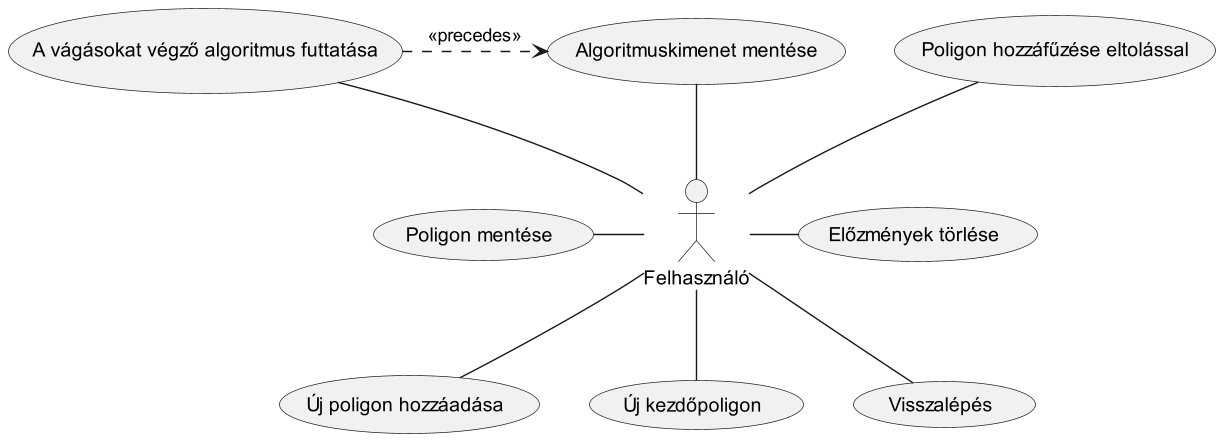
\includegraphics[width=1\linewidth]{images/usecase_editor_actions.png}
    \caption{Szerkesztői műveletek felhasználói esetek}
    \label{fig:usecase_editor_actions-1}
\end{figure}

\subsection{Poligon műveletek}

A poligon tartalmának módosítására létrehozott műveletek találhatóak a szekción belül.

\begin{figure}[H]
    \centering
    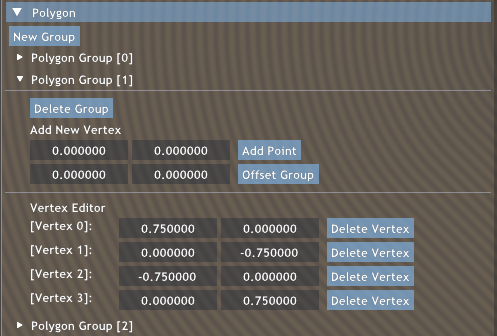
\includegraphics[width=0.85\linewidth]{images/polygon_actions.png}
    \caption{Poligon műveletek GUI}
    \label{fig:polygon_actions-1}
\end{figure}

\textbf{Elérhető funckionalitás}

\begin{description}
    \item[Új csoport hozzáadása] Egy új alpoligon kerül hozzáadásra. Az új csoport felhasználható lyukak vagy további elkülönülő alakzat elkészítésére.
    \item[Csoport > Csoport törlése] Törli az adott csoportot, azzal a feltétellel, hogy egy poligonban legalább egy csoportnak szerepelnie kell.
    \item[Csoport > Csúcs hozzáadása] A megadott pozícióval hozzáad egy csúcspontot a csoport végére.
    \item[Csoport > Csoport eltolása] A megadott pozícióval eltolja minden csúcsát a csoportnak.
    \item[Csoport > Csúcs > Törlés] Eltávolítja az adott csúcsot.
\end{description}

\begin{figure}[H]
    \centering
    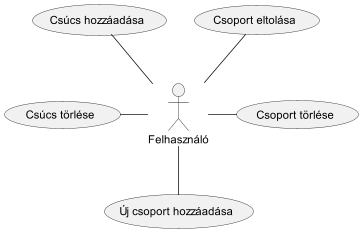
\includegraphics[width=.6\linewidth]{images/usecase_polygon_actions.png}
    \caption{Poligon műveletek felhasználói esetek}
    \label{fig:usecase_polygon_actions-1}
\end{figure}

\subsection{Eseménynapló}

A szerkesztés során számos esemény kerül kiváltásra különböző források hatására. Az eseménynaplóban megvizsgálhatunk minden bejövő eseményt valós időben. Az ismétlődő szignatúrák számozással csoportosításra kerülnek, mivel bizonyos esetekben másodpercenként akár több tíz is kiváltódhat, például amikor a felhasználó az egérrel mozgat egy csúcspontot, vagy egy alpoligont.

\begin{figure}[H]
    \centering
    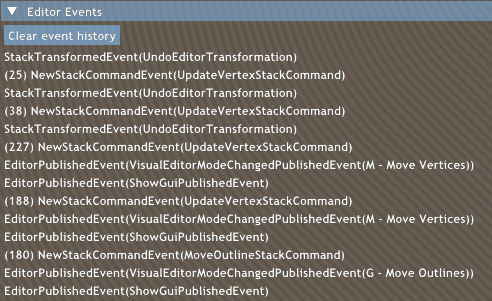
\includegraphics[width=1\linewidth]{images/editor_events.png}
    \caption{Poligon műveletek GUI}
    \label{fig:editor_events-1}
\end{figure}

\textbf{Elérhető funckionalitás}

\begin{description}
    \item[Napló törlése] Az összes bejegyzés törlése a naplóból.
\end{description}

\section{Vizuális szerkesztő}\label{sec:visual_editor}

A vizuális szerkesztő lehetőséget ad arra, hogy szabadkézzel szerkesszük a sokszögünket. Billentyűzet segítségével válthatunk módok (eszközök) között, majd az egérrel interakcióba léphetünk a poligonnal vagy a vászonnal. A vizuális szerkesztőn keresztül válthatunk a háromdimenziós nézetre is.

\textbf{Elérhető funckionalitás}

\begin{description}
    \item[Csúcspontok mozgatása (M billentyű)] Csúcspontok mozgatása "Drag and drop". Egérgomb lenyomásakor a program kiválasztja a legközelebbi csúcspontot egy megadott távolságkorláton belül és mozgatás hatására frissíti a pozíciójat.
    \item[Csoportok mozgatása (G billentyű)]  Csoportok mozgatása "Drag and drop". Egérgomb lenyomásakor a program kiválasztja a legközelebbi csúcsponthoz tartozó csoportot egy megadott távolságkorláton belül és mozgatás hatására frissíti a csoportban lévő csúcspontok pozícióját.
    \item[Vászon mozgatása (V billentyű)] Az egérgomb nyomvatartásával és mozgatással mozgatni lehet a vászonon a teljes poligont. A görgő segítségével pedig nagyítani és zsugorítani a méretén. Ez a művelet nem módosít a poligon állapotán.
    \item[Csúcspont beszúrása (I billentyű)] A bal egérgomb lenyomásával elhelyez egy csúcspontot a kattintás pozíciójához legközelebbi kettő, azonos csoporthoz tartozó csúcspont közé. A jobb egérgomb lenyomásával a legközelebbi csúcspont törlésre kerül, amennyiben egy megadott távolságon belül van.
    \item[Váltás a háromdimenziós algoritmus kimenet nézetre (D billentyű)] Ha az algoritmus végrehajtásra került a poligon jelenlegi állapotán, akkor átvált a háromdimenziós nézetre, egyébként egy felugró ablakban jelzi, hogy nincs mit megjeleníteni.
\end{description}

\begin{figure}[H]
    \centering
    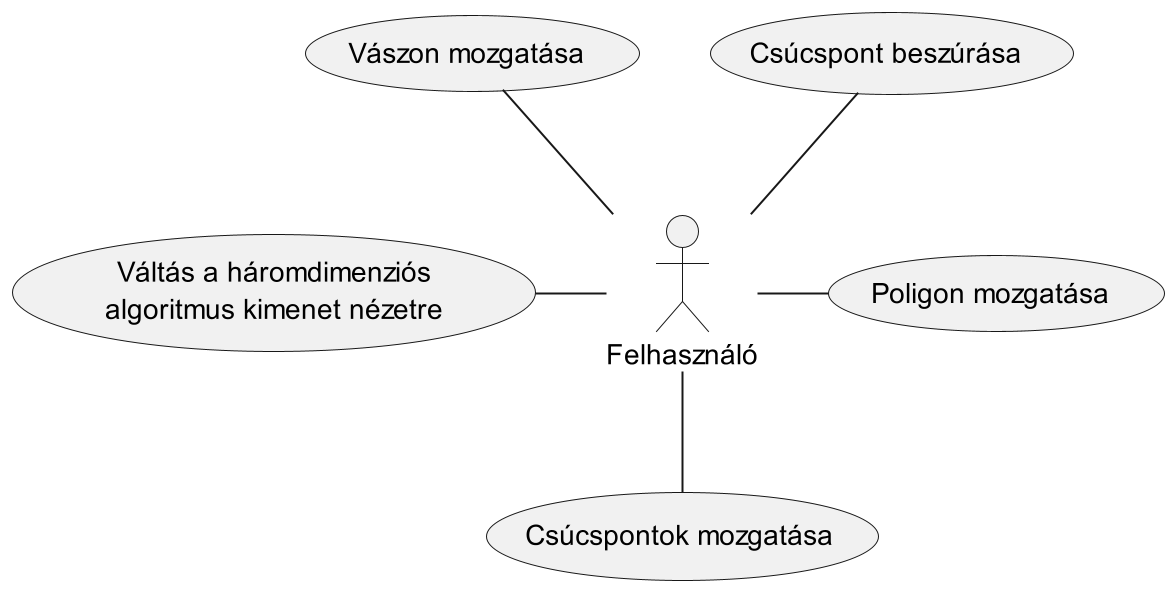
\includegraphics[width=.7\linewidth]{images/usecase_visual_editor.png}
    \caption{Vizuális szerkesztő felhasználói esetek}
    \label{fig:usecase_visual_editor-1}
\end{figure}

\section{Poligon háromdimenziós nézete}

Az algoritmus kimenetével egy háromdimenziós objektumként számol az alkalmazás megjelenítéskor, ahol a mélységi komponens az előjeles távolság abszolútértéke. Ezt a tulajdonságot kihasználva ebben a nézetben a térben mozgatva tekinthetjük meg poligonunkat.

Ebben az állapotban nem szerkeszthető a poligon, ezért a teljes GUI el van rejtve. A szerkesztői felületre bármelyik \ref{sec:visual_editor}-ban említett eszközhöz rendelt billentyű lenyomásával átválthatunk.

\begin{figure}[H]
    \centering
    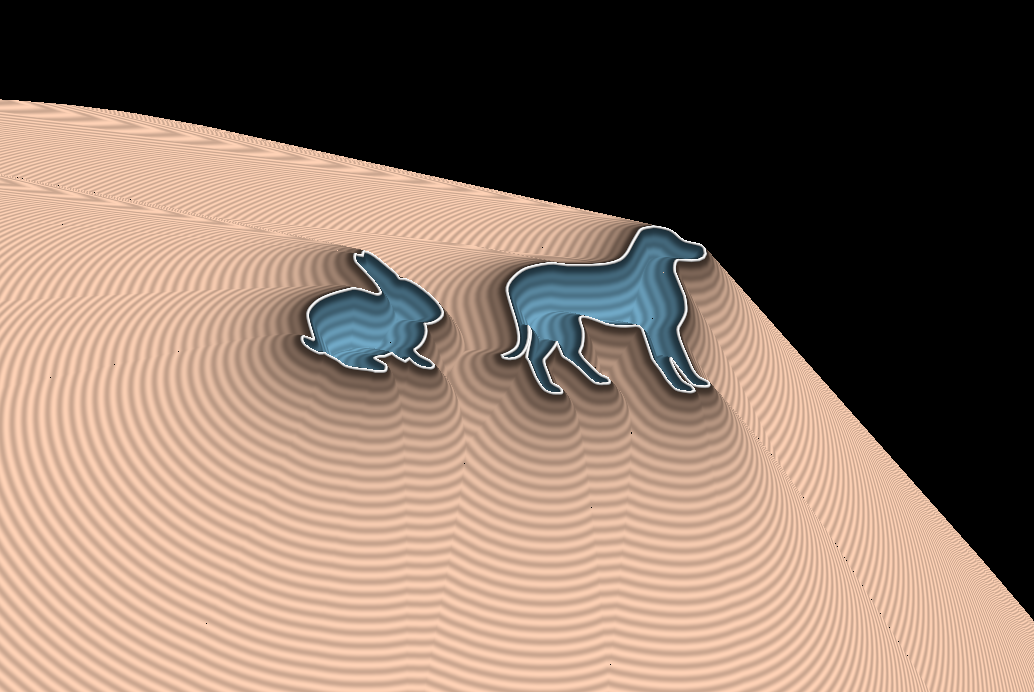
\includegraphics[width=1\linewidth]{images/3d_view.png}
    \caption{Poligon háromdimenziós nézete}
    \label{fig:3d_view-1}
\end{figure}

A görgő segítségével változtathatjuk a távolságot a kamera és az objektum közepe között. Az egérgomb lenyomvatartása és mozgatással pedig forgathatjuk a geometriát, a mozgatás horizontális komponensével az Y tengey körül, a vertikális komponenssel pedig az X tengely körül.
